%%%%%%%%%%%%%%%%%  Debut du fichier Latex  %%%%%%%%%%%%%%%%%%%%%%%%%%%%%%
\documentclass[letterpaper,12pt,onecolumn]{article}

%%% Pour un texte en francais

%%\usepackage[applemac]{inputenc}
%\usepackage[francais]{babel}
	         % encodage des lettres accentuees
\usepackage[T1]{fontenc}
\usepackage[utf8]{inputenc}          % encodage des lettres accentuees
%\usepackage{graphicx}
%%\usepackage{graphicx} \def\BIB{}
\usepackage[paper=a4paper,left=2.1cm,right=2.1cm,top=2.5cm,bottom=2.5cm]{geometry}
\usepackage{multicol}
\usepackage{graphicx,wrapfig,lipsum} 
%\def\BIB{}
\usepackage{caption}
\usepackage{subcaption}
\usepackage[pdftex]{hyperref}
%\usepackage{natbib}
\usepackage{url}
\usepackage{perpage} %the perpage package
\MakePerPage{footnote} %the perpage package command
\hypersetup{
    colorlinks,%
    citecolor=black,%
    filecolor=black,%
    linkcolor=black,%
    urlcolor=blue     % can put red here to visualize the links
}

\usepackage{enumitem}
\usepackage{amssymb}

%\renewcommand{\refname}{}

\usepackage{floatrow}

\usepackage{fancyhdr}
\usepackage{lastpage}

\pagestyle{fancy}
\fancyhf{}
\rhead{Research summary}
\lhead{El Mellah Ileyk}
\rfoot{\thepage / \pageref{LastPage}}

\DeclareUnicodeCharacter{00A0}{ }

\usepackage{xspace}

%%% Quelques raccourcis pour la mise en page
\newcommand{\remarque}[1]{{\small \it #1}}
\newcommand{\rubrique}{\bigskip \noindent $\bullet$ }
\newcommand{\sgx}{SgXB\xspace}
\newcommand{\ulx}{ULX\xspace}
\newcommand{\sfxt}{SFXT}
\newcommand{\sg}{Sg\xspace}
\newcommand{\co}{CO\xspace}
\newcommand*{\hmxb}{HMXB\@\xspace}
\newcommand*{\lmxb}{LMXB\@\xspace}
\newcommand*{\rlof}{RLOF\@\xspace}
\newcommand*{\ns}{NS\@\xspace}
\newcommand*{\bh}{BH\@\xspace}
\newcommand*{\eg}{e.g.\@\xspace}
\newcommand*{\ie}{i.e.\@\xspace}
\newcommand*{\aka}{a.k.a. \@\xspace}
\newcommand*\diff{\mathop{}\!\mathrm{d}}
\newcommand{\mystar}{{\fontfamily{lmr}\selectfont$\star$}}
\newcommand*{\msun}{$M_{\odot}$\@\xspace}
\newcommand*{\mdotstar}{$\dot{M}_{\text{\mystar}}$\@\xspace}
\newcommand*{\mdotacc}{$\dot{M}_{\text{acc}}$\@\xspace}
\newcommand*{\ledd}{$L_{\text{Edd}}$\@\xspace}


\newcommand{\ignore}[1]{}

%\renewcommand*\rmdefault{iwona}

%\pagenumbering{gobble}

%\bibliographystyle{abbrvnat}
%\setcitestyle{authoryear,open={((},close={))}}

%\renewcommand{\thefootnote}{\roman{footnote}}

% -------------------------------------------------
\newcommand{\horrule}[1]{\rule{\linewidth}{#1}} % Create horizontal rule command with 1 argument of height

\title{	
\vspace*{-2.5cm}
%\normalfont \tiny 
%%\textsc{Paris Diderot} \\ [25pt] % Your university, school and/or department name(s)
%\horrule{0.5pt} \\[0.4cm] % Thin top horizontal rule
\Large Speeding up the spinning top\\
\large How accretion sets the pace in High Mass X-ray Binaries  \\ % The assignment title
%\horrule{2pt} \\[0.5cm] % Thick bottom horizontal rule
}
\author{\tiny} % Your name
\date{\tiny }%\normalsize\today} % Today's date or a custom date
% -------------------------------------------------

%\makeatletter
%\def\@xfootnote[#1]{%
%  \protected@xdef\@thefnmark{#1}%
%  \@footnotemark\@footnotetext}
%\makeatother

\usepackage[square,numbers,sort]{natbib}
%\usepackage{har2nat} % "natbib" is loaded automatically

%
%\let\oldthebibliography\thebibliography
%\renewcommand{\thebibliography}[1]{%
%  \oldthebibliography{#1}
%  \let\oldbibitem\bibitem
%  \let\oldtextsc\textsc
%  \def\oldbbland{et}
%  \newcounter{authorcount}
%  \def\bibitem[##1]##2{%
%    \let\textsc\oldtextsc
%    \let\bbland\oldbbland
%    \oldbibitem[##1]{##2}%
%    \let\textsc\mytextsc%
%    \let\bbland\mybbland
%    \setcounter{authorcount}{0}
%  }
%  \def\mybbland{\setcounter{authorcount}{0}\oldbbland}
%  \def\dropetal##1.{ \bbletal}
%  \def\mytextsc##1{%
%    \oldtextsc{##1}%
%    \stepcounter{authorcount}%
%    \ifnum\value{authorcount}=2\relax%
%      \expandafter\dropetal%
%    \fi%
%  }%
%}


\begin{document}

%\bibpunct{[}{]}{;}{n}{,}{,}

%%%%%%%%%%%%%%%%%%%%%%%%%  PREMIERE PAGE %%%%%%%%%%%%%%%%%%%%%%%%%%%%%%
%%% DANS CETTE PAGE, ON REMPLACE LES INDICATIONS ENTRE CROCHETS [...]
%%% PAR LES INFORMATIONS DEMANDEES
%%%%%%%%%%%%%%%%%%%%%%%%%%%%%%%%%%%%%%%%%%%%%%%%%%%%%%%%%%%%%%%%%%%%%%%

\renewcommand{\headrulewidth}{1pt}
\pagestyle{fancy}
\fancyhf{}
\rhead{Research proposal}
\lhead{El Mellah Ileyk}
\rfoot{\thepage / \pageref{LastPage}}

\vspace*{-1.2cm}
\begin{center}
\Large \textbf{Speeding up the spinning top}\\
\large How accretion sets the pace in High Mass X-ray Binaries 
\end{center}
\normalfont

%\vspace*{0.7cm}

%Massive stars live a forceful life during which they shape galaxies with their mechanical, radiative and chemical feedback. Most of them evolve in a binary system where the two stars orbit close enough from each other to exchange mass, angular momentum and sometimes merge during their evolution \citep{DeMink2012}. Those who remain bounded after the supernova explosion of one the two objects can become a High Mass X-ray Binaries (\hmxb), systems where stellar material is transferred to the compact remnant, either a neutrons star (\ns) or a black hole (\bh). This temporary albeit decisive period in the binary evolution determines its final fate, once a compact binary is formed.
%
%The recent detection of gravitational waves granted us access to the very last moment of this epic journey : the coalescence between two compact objects. It revealed the final masses and effective spins the \bh and \ns involved acquired during their turbulent lifetime \citep{TheLIGOScientificCollaboration2017}. These systems are thought to be the fruit of a massive binary evolution which can lead, under stringent conditions, to compact binaries with orbital separations close enough to spiral-in and merge within a Hubble time. 

Massive stars live a forceful life during which they shape galaxies with their mechanical, radiative and chemical feedback. Most of them evolve in a binary system where the two stars orbit close enough to strongly interact and sometimes merge during their evolution \citep{DeMink2012}. Last year, a gravitational wave detection granted us access to the very last moment this epic journey can lead to: the coalescence between two neutron stars (\ns), which unveiled the final masses and spins they acquired during their turbulent lifetime \citep{TheLIGOScientificCollaboration2017}. An intermediate step between these two stages are High Mass X-ray Binaries (\hmxb), systems where stellar material is transferred from an evolved massive star to an orbiting compact remnant. The conditions of this transfer determine whether a double \ns with an orbital separation small enough to spiral-in and merge within a Hubble time will eventually be formed. 

%\begin{wrapfigure}{o}{0.6\textwidth}
%  \centering
%  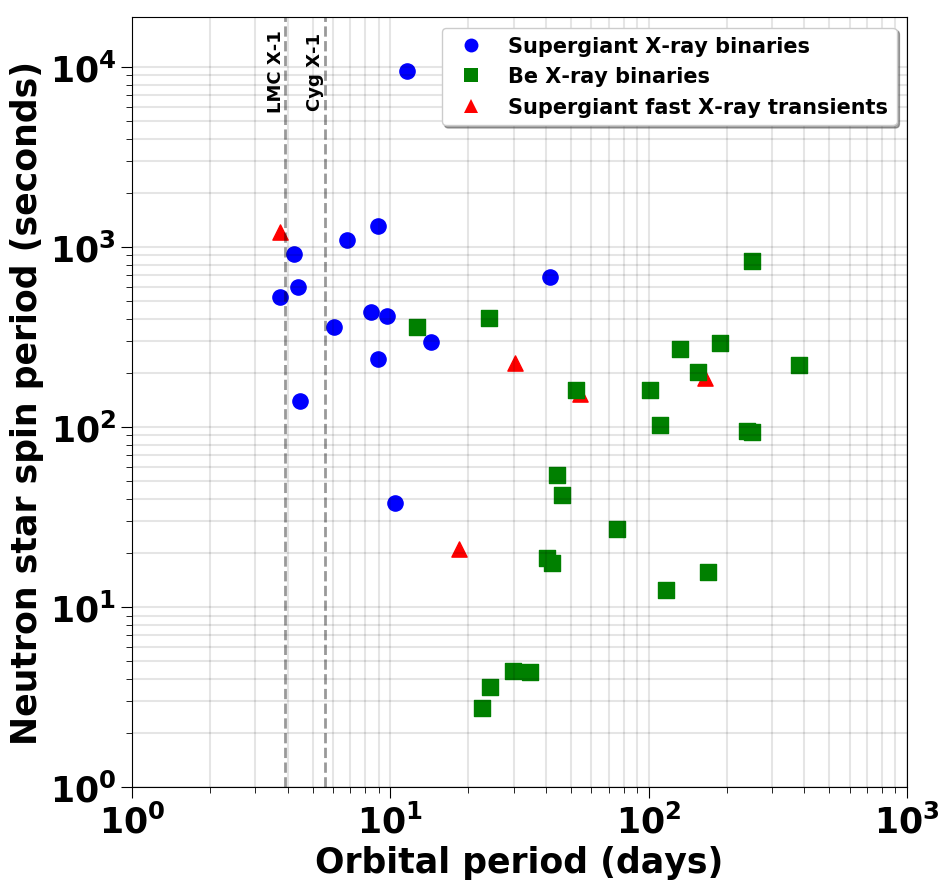
\includegraphics[width=0.6\textwidth]{Figures/corbet_diag.png}
%  \caption{3D contours of the mass density, where the arrows stand for the velocity field in the orbital plane. The central white sphere stands for the inner boundary of the simulation space which represents approximately the outer edge of the \ns magnetosphere, a few 100 times smaller than the outer boundary of the simulation space.}
%  \vspace{-10pt}
%\label{fig:disc}
%\end{wrapfigure}

%\begin{wrapfigure}{o}{0.6\textwidth}
%  \centering
%  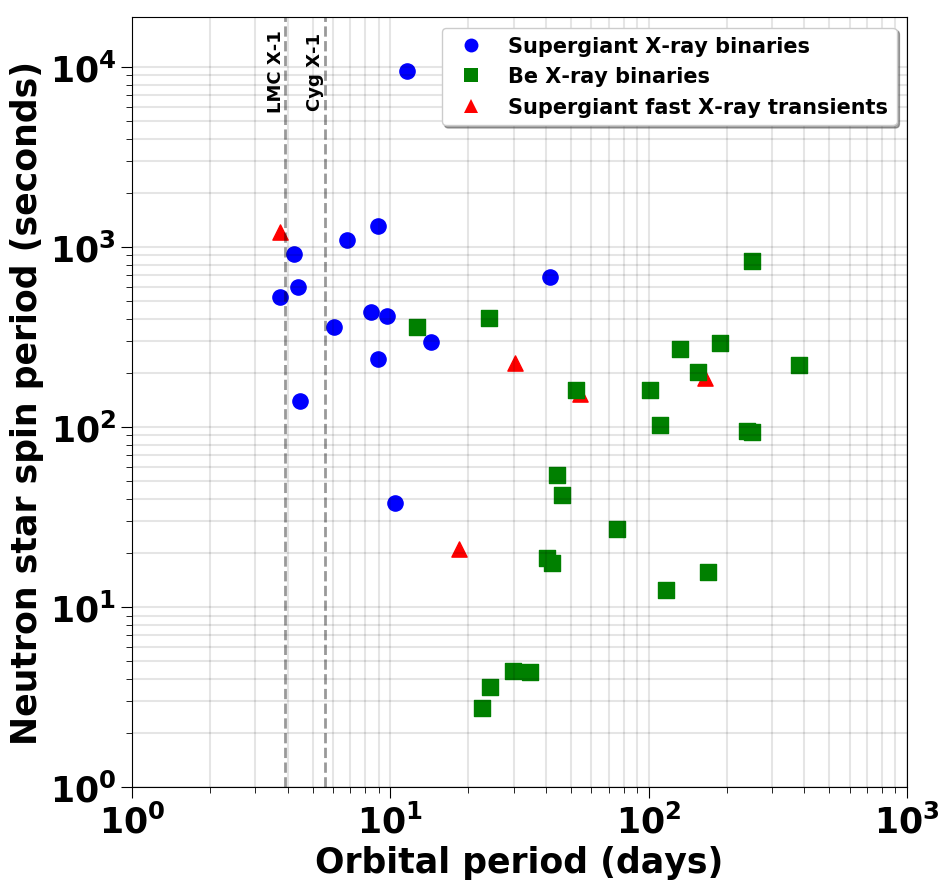
\includegraphics[width=0.6\textwidth]{Figures/corbet_diag.png}
%  \caption{3D contours of the mass density, where the arrows stand for the velocity field in the orbital plane. The central white sphere stands for the inner boundary of the simulation space which represents approximately the outer edge of the \ns magnetosphere, a few 100 times smaller than the outer boundary of the simulation space.}
%  \vspace{-10pt}
%\label{fig:disc}
%\end{wrapfigure}

Loss and exchange of angular momentum during this phase is a key problem to address. \ns are surrounded by an extended magnetosphere plays a major role in the accretion process: the spin of the \ns in \hmxb perturbs the accretion through magneto-centrifugal effects and episodic mass outflows \citep{Bozzo2008}. Furthermore, the orbital separation has a direct impact on the mass transfer mechanism (Roche lobe overflow or wind accretion), on the geometry of the accretion flow and on the subsequent spiral-in time. Models are being developed to describe the formation of double \ns systems \citep{Tauris2017} but thorough and repeated observations of individual \hmxb remind us how uncertain the proxies we rely on to compute evolutionary tracks can be. The distinction between the limit disc and wind-fed regimes prevents us from treating the realistic intermediate case, with a stellar wind significantly beamed towards the accretor much before stellar evolution leads to stellar Roche lobe overflow. Within the current uncertainties on the properties of the winds of evolved massive star (mass loss rate, velocity profile, micro-structure), the geometry of the accretion flow when it reaches the magnetosphere fluctuates \citep{ElMellah2018}. Since the instantaneous torques at stake depend on whether the material forms a thin disc (prograde or retrograde) or remains essentially spherical as it is accreted, it has dramatic consequences on the spinning up or down of the accretor \citep{Ghosh1978,Shakura2012}. 

%The spin of the \ns itself can also perturb the accretion through magneto-centrifugal effects and episodic mass outflows \citep{Bozzo2008}. 

A good illustration of our incomplete understanding is given by the distribution and evolution of the \ns spin in Supergiant X-ray binaries (\sgx, a sub-class of \hmxb, see Figure\,\ref{fig:spin}). While some sub-classes of \hmxb show common angular momentum trends, wind accreting \ns in \sgx still defy theoretical expectations. They can display distinct long term phases of spinning up or down, which prove that the torque does not obey a random walk, and torque reversals are not necessarily associated to spectral or flux variations \citep{Hemphill2013}. 

%Instantaneous torques are the result of intertwined effects: depending on whether the accreted material forms a thin disc (prograde or retrograde) before reaching the \ns magnetosphere or remains essentially spherical, the torque applied to the \ns is significantly different \citep{Ghosh1978,Shakura2012}. However, the spin of the \ns itself can perturb the accretion through magneto-centrifugal effects \citep{Bozzo2008} while the properties of the stellar wind captured determines the geometry of the flow once it reaches the outer rim of the magnetosphere \citep{ElMellah2018}. 

The aim of this project is to gather these torque mechanisms into a consistent frame to evaluate the loss and transfer of angular momentum in the complex environment of \ns-hosting \sgx following these core questions:

%For accreting \bh, the contribution of ejection via jets or disc winds does not simplify the picture. 

%The omnipresence of this type of feedback loops in \hmxb between similarly important effects demands to design models where scales are connected and tackle simultaneously the core questions of this project :

%Finally, the X-rays produced as the flow is captured alter the properties of the stellar wind upstream. 

%results of the interaction between the wind of the donor star,  the magnetosphere of the \ns or

%The question of the angular momentum accretion rate onto the compact object is of uttermost importance to 
%is not settled yet.
% far from being solved.

%Dips, off-states, flares, hardening and other short term variability accessible to observational campaigns : our limited understanding of their origin (discs, shocks, jets, large or small scale structures passing by the line-of-sight...) puts at risk the steady picture from which we try to extrapolate the secular evolution.

%In particular, t

%We need to understand how angular momentum was lost and transferred during the \hmxb phase to predict the frequency of compact objects mergers and trace back their tumultuous history. 
%
%To do so, the project will focus on the following core questions :

\begin{enumerate}
\item[\textbf{Q1.}] How does the flow connect to the magnetosphere and what are the short and long term consequences for the spin of the \ns? 
\item[\textbf{Q2.}] How does radiative heating/cooling influence the flow geometry at the magnetosphere?
\item[\textbf{Q3.}] How does the partial capture of stellar material by the \ns alter the orbital separation and how does it retroactively impact the stellar mass loss?
\end{enumerate}

\begin{figure}[!h]
\centering
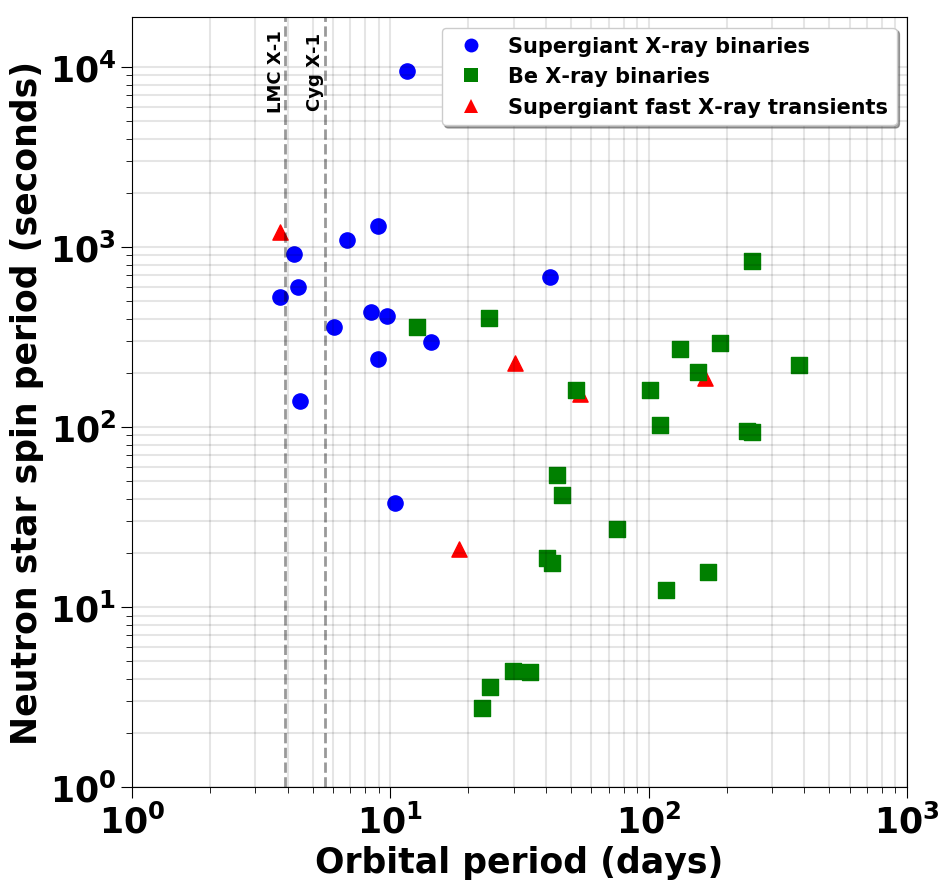
\includegraphics[width=0.7\columnwidth]{Figures/corbet_diag.png}
\caption{\ns-hosting Galactic \hmxb with known orbital and \ns spin periods. While a correlation exists between the spin and the orbital period in X-ray binaries where the donor star is a massive Be star (a fast rotator surrounded by a decretion disc), it is not the case in \sgx or in Supergiant fast X-ray transients.}
\label{fig:spin}
\end{figure} 

\begin{figure}[!h]
\vspace*{0.3cm}
\floatbox[{\capbeside\thisfloatsetup{capbesideposition={right,center},capbesidewidth=5cm}}]{figure}[\FBwidth]
{\caption{Color map slice of the density in the equatorial plane and 3D iso-density surface. The accretor lies in the center and the wind comes from the bottom left. The capture of an overdense "clump" of matter is visible. The solid white line delimits the envelope of the shocked region, perturbed by clumps. The clump carries enough angular momentum to form a transient disc-like structure around the \ns magnetosphere, engulfed in the flow.}\label{fig:disc}}
{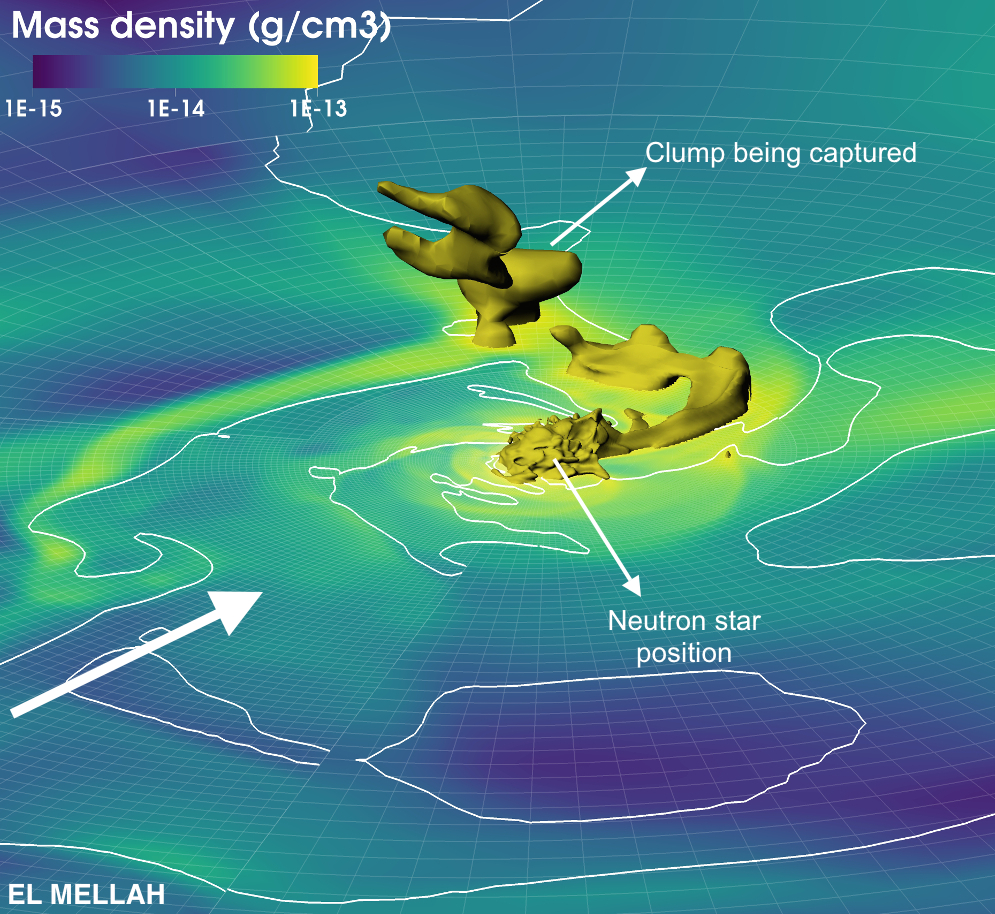
\includegraphics[width=11cm]{Figures/clump_intruder.jpeg}}
\vspace*{-0.4cm}
\end{figure}

Until now, the several orders of magnitude which separate the orbital scale from the X-ray emitting region, in the immediate vicinity of the compact object, have precluded any bold numerical attempt to follow the accreted flow all along its journey. We were condemned to compute the torques applied by ad-hoc  accretion geometries, presupposing an idealized behavior of the scales out of the scope of the simulation. Within an active collaboration which gathered 20 to 30 observers and theoreticians of winds of massive stars and X-ray binaries over the last years, I have developed and validated a numerical framework which connects these scales and offer the first comprehensive view of mass transfer via line-driven winds to compact accretors in binaries. I am now in a position to step forward and investigate the torques associated.


% to solve the radiative magneto-hydrodynamics (RMHD) equations in neatly designed numerical setups. Based on the ample experience I have acquired with these tools, I can reasonably aspire to bring new insights on these questions and contribute to put the newly born field of gravitational wave astronomy into perspective.
%
%I have gained extensive expertise over the last 5 years with highly parallel finite volume codes to solve the 3D MHD equations in non-Cartesian geometries and performed computationally-demanding simulations on Tier-1 supercomputers. 

%\subsection*{Observational motivations}
%
%If mergers of compact objects set the final state, the simulations I intend to develop feed on observations of the instantaneous state of \hmxb. That is why I have been leading my studies hand in hand with observers, to guarantee the relevance of the numerical setups I designed. The plethora of \hmxb observations carried out thanks to the X-ray instruments in orbit identified the main structures to be modeled in these systems. Orbital-phase resolved spectroscopy performed with the NASA Chandra satellite and the ESA XMM-Newton satellite revealed zones of enhanced ionization and enhanced absorption events \citep{Martinez-Nunez2014,Grinberg2017}. My numerical investigations aim at capturing the dynamics underlying this complex geometry : they disentangle between transient features such as episodic flares due to the micro-structure of the wind \citep{ELMELLAH2017}, and recurring events associated to stable structures present from orbit to orbit such as the bow shock surrounding the accretor \citep{ELMELLAH2015}. The evolution of the spin of the compact object obeys the same logic of systematic and contingent evolution. Although the mass accretion rate might vary little with the geometry of the flow, the long term impact on the torque applied to the compact object can be dramatic. Key simulation parameters are also supplied by the available instruments : in \hmxb hosting a \ns, the observation of cyclotron resonance scattering features with the NASA NuSTAR satellite \citep{Furst2014} sets constrains on the extent of the magnetosphere of direct interest to define representative numerical models of spinning up/down. The wealth of observational data enables us to set a reliable simulation stage to investigate further the coupling between the two spins and the orbital angular momentum via wind accretion and interpret the refined observations of future X-ray satellites.

%INTRODUCE SPIN : MEASURED IN LMXB AND AGN (REF).

%\begin{figure}[!b]
%\centering
%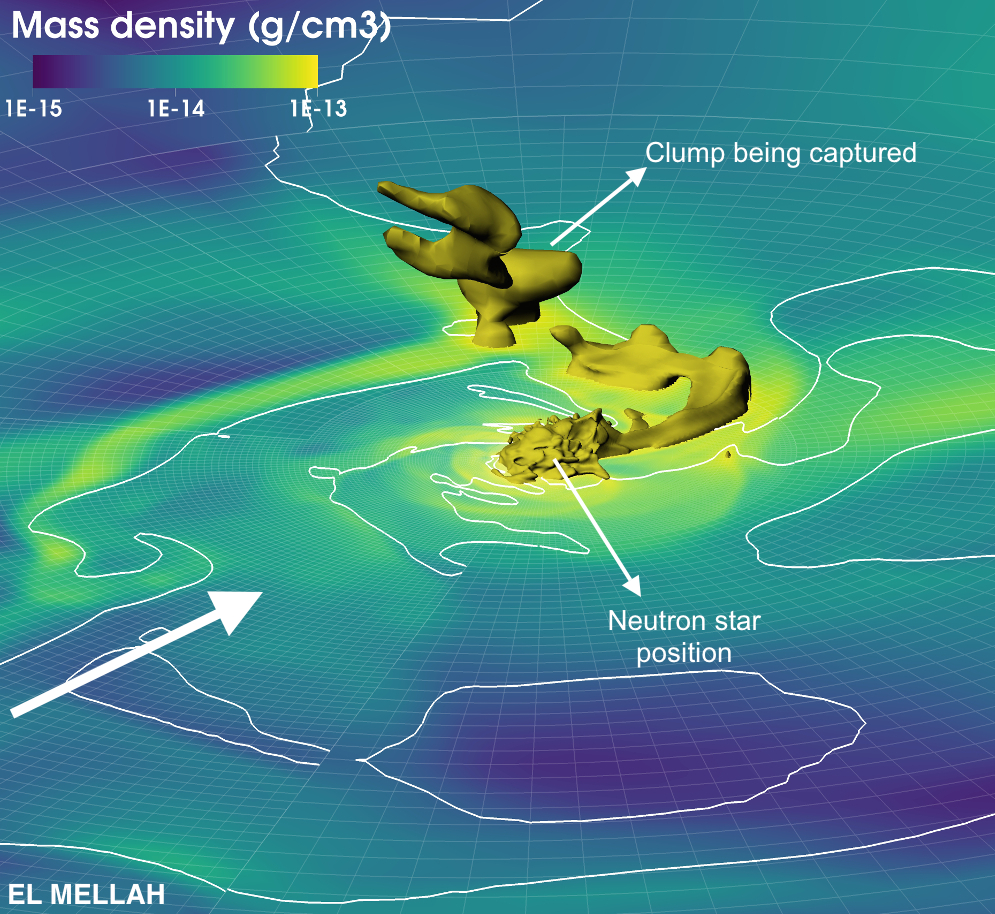
\includegraphics[width=0.65\columnwidth]{Figures/clump_intruder.jpeg}
%\caption{Color map slice of the density in the equatorial plane and 3D iso-density surface. The solid white line delimits the Mach-1 surface in the equatorial plane. The accretor lies in the center and the wind comes from the direction bottom left. The capture of an overdense "clump" of matter is visible. The clump carries enough angular momentum to form a transient disc-like structure around the \ns magnetosphere, engulfed in the flow.}
%\label{fig:disc}
%\end{figure} 

\subsection*{Methodology}

As a computational astrophysicist, the underlying tools of my research are models based on observations and detailed numerical simulations. I have gained ample experience over the last five years with cutting-edge massively parallel codes to solve the 3D magneto-hydrodynamics equations in non-Cartesian geometries and I have performed computationally-intensive simulations on Tier-1 supercomputers. On the other hand, I also embraced the diversity of structures and environments highlighted by observers in the numerical setups I designed: I treat, within the same simulation space, zones of enhanced ionization or density \citep{ElMellah} and the accretion tail \citep{ElMellah2015} identified by orbital-phase resolved spectroscopy of the classic \sgx Vela X-1 with the NASA Chandra satellite \citep{Grinberg2017} and the ESA XMM-Newton satellite \citep{Martinez-Nunez2014} respectively. I can now address the entry of the accretion flow in the \ns magnetosphere and its consequences on the transfer of angular momentum through the following steps. Notice that although they would profit from each other, these steps are autonomous enough to be performed separately, may one of them not unfold as planned.

\begin{itemize}[label={\rotatebox[origin=c]{180}{$\Lsh$}}]
\item \textbf{\underline{Step 1: Flow-magnetosphere boundary layer}} I could first make use of the representative flow geometries I identified in \citep{ElMellah2018} (spherical, thin or thick disc, prograde or retrograde) to study the encounter between the inflowing material and the \ns magnetosphere. The net spinning up or down associated to each regime would be computed in a full 3D time-dependent environment. I would measure the capacity of the flow to penetrate the magnetosphere via magnetic reconnection, relying on observational parameters (\eg the magnetic moment deduced from observations of cyclotron resonance scattering features with the NASA NuSTAR satellite \citep{Furst2014}). This step would also serve to refine the numerical setup (identification of appropriate adaptive mesh refinement criteria to reach numerical convergence, validation of the magnetic divergence cleaning tools already available in \texttt{MPI-AMRVAC}...). The torques measured in these simulations depending on the geometry and their comparison to reported values in \sgx would be reported in a first publication addressing \textbf{Q1}.
\item \textbf{\underline{Step 2: Radiative feedback}} \textit{This step is subdivided in an implementation step (a) and two physical applications steps which would lead to a paper each (b linked to \textbf{Q2} and b' linked to \textbf{Q3}).} \textit{(a)} The formation of a disc depends on the capacity of the flow to radiate away its internal energy and compress. I implemented a first cooling prescription and used cooling modules suitable for radiatively thin environments, but I now intend to rely on the more realistic treatment of radiative effects available in the \texttt{FLASH} or the \texttt{HARMRAD} codes used by several teams in the US \citep{McKinney2014}. A side application, suitable for a one-year graduate project, would be the extraction of photometric and spectroscopic synthetic observations from the simulations to be confronted to the observations. \textit{(b)} For a spherical accretion flow, the rate of plasma entering into the magnetosphere is determined by the interchange instability \citep{Shakura2012}. The latter is triggered by Compton cooling of the hot plasma as it interacts with the X-rays from the accretor. \textit{(b')} An inspiralling \ns could in theory eject the envelope of its massive star companion \citep{Kruckow2016}. With the proper radiative treatment developed in \textit{(a)}, 3D radiative-hydrodynamics simulations of common envelope ejection including regions where the luminosity reaches the Eddington luminosity could be performed. It would be an unprecedented computation of the efficiency of the envelope unbinding, a key parameter to evaluate the fraction of mergers of compact binaries susceptible to be detected \citep{Murguia-Berthier2017}.
\item \textbf{\underline{Step 3: Transitions and duty cycle}} making use of the multi-scale setup I developed, I could investigate how the micro-structure of the wind provoke stochastic variations of the geometry (\eg in Figure\,\ref{fig:disc}) susceptible to make the accretion regime transit from a stage to another (\eg activation of the propeller effect or inversion of the disc rotation). Longer simulations would estimate the duty cycle of the torques and the net spinning up or down of the \ns. In a publication addressing \textbf{Q1} from a complementary point of view, I could confront the first synthetic curves of the evolution of the \ns spin as a function of time to the observed ones (\eg in the wind-fed \ns Ultra-luminous X-ray source, P13 ULX-1, whose pulse period derivative remains to be explained, \citep{Fuerst2018}). Perspectives to extend the present project would naturally arise, with the possibility to investigate the impact of these new results on the secular evolution of these systems.
\end{itemize}

%The ample experience I have acquired with 
%
%Kruckow2016
%\cite{Murguia-Berthier2017}
%
%I would devote 
%
%, adapting cutting edge massively parallel codes: . Based on the ample experience I have acquired with these tools, I can reasonably aspire to 
%
%to solve the radiative magneto-hydrodynamics (RMHD) equations in neatly designed numerical setups
%
%For radiation-dominated environments, I intend to couple this code to available solvers based either on flux-limited diffusion or M1 radiative closure. It will make the implementation reusable for projects beyond the current one (\eg the question of torques in super-Eddington accretion situations).
%
%I propose to investigate transfer and loss of angular momentum in \hmxb using RMHD numerical simulations of situations tightly linked to observational signatures. For instance, orbital-phase resolved spectroscopy performed with the NASA Chandra satellite and the ESA XMM-Newton satellite identified the main structures which need to be treated in models of \hmxb (\eg zones of enhanced ionization \citep{Grinberg2017}, accretion tail \citep{Martinez-Nunez2014}...). My numerical investigations aim at capturing the dynamics underlying this complex geometry: they disentangle between stochastic features such as transient discs due to the micro-structure of the wind (see Figure\,\ref{fig:disc} from \cite{ElMellah}), and recurring events associated to stable structures present from orbit to orbit such as the accretion tail in the wake of the accretor \citep{ElMellah2015}.

%\begin{itemize}
%\item \textbf{\underline{Step 1: Radiative feedback}} The geometry of the problem (\eg formation of an accretion disc) strongly depends on the capacity of the flow to radiate away its internal energy and compress. Although the mass accretion rate might vary little with the geometry of the flow, the long term impact on the torque applied to the compact object can be dramatic. I implemented a first cooling prescription and used cooling modules suitable for radiatively thin environments, but I now intend to rely on the more realistic treatment of radiative effects available in the \texttt{FLASH} or the \texttt{HARMRAD} codes used by several teams in the US \citep{McKinney2014}. It will also enable me to extract photometric and spectroscopic synthetic observations from the simulations to be confronted to the observations. 
%%For instance, a first publication would assess the possibility for transient truncated discs around \ns to contribute to the soft-excess observed in \ns-\sgx \citep{Bozzo2012}.
%\item \textbf{\underline{Step 2: Coupling with the \ns magnetosphere}} Once the impact of radiative feedback on the geometry is known, we can make use of the multi-scale setup I developed and evaluate, in realistic conditions, the net spinning up or down of a wind-fed \ns. We have semi-analytical expectations for the limit cases, spherical or thin disc geometry, but we can now treat the full 3D time-dependent problem to draw conclusions about the systematic effects which need to be accounted for in computation of population synthesis. In a publication, I could confront the first synthetic curves of the evolution of the \ns spin as a function of time to the observed ones (\eg in the \ns-hosting Ultra-luminous X-ray source P13 which remain to be explained, \citep{Fuerst2018}). In specific \sgx like Vela X-1, key simulation parameters such as the extent of the magnetosphere are provided by observations of cyclotron resonance scattering features with the NASA NuSTAR satellite \citep{Furst2014}.
%\item \textbf{\underline{Step 3: The role of outflows}} Stellar winds are an important source of angular momentum loss in \sgx, along with disc winds and jets in some systems like Cygnus X-1: accretion-ejection in the disc via magneto-centrifugal effects are possible (\eg a Blandford-Payne disc wind) while Blandford-Znajek jets damp the \bh spin in a different way for a prograde or a retrograde disc \citep{Tchekhovskoy2012}. Also, the ejection of stellar material during the common envelope phase can significantly alter the long term evolution of the spins and orbital separation \cite{Murguia-Berthier2017}. If I am granted a Hubble fellowship, the team I would eventually join will influence which aspect I focus more on in this third step. Depending on the skills and centers of interest of the host institution I would be endorsed by, I would set the focus either on the role of outflows in spinning down a wind-fed \bh or on the efficiency of stellar material ejection in the common envelope phase.
%\end{itemize}

%I will build up my models hand in hand with 
%
%Step 1 : radiative coupling (ionization of the wind and heating of the inflow => thickness of the disc)
%Step 2 : magnetic component : magnetosphere (produce Pdot diagrams for NS) and turbulent (MRI)
%Step 3 : outflows (MAD, jets...)

%\subsection*{Computational tools}
%
%I have gained extensive expertise over the last 5 years with highly parallel finite volume codes to solve the 3D MHD equations in non-Cartesian geometries and performed computationally-demanding simulations on Tier-1 supercomputers. 
%
%For radiation-dominated environments, I intend to couple this code to available solvers based either on flux-limited diffusion or M1 radiative closure. It will make the implementation reusable for projects beyond the current one (\eg the question of torques in super-Eddington accretion situations).
%
% \texttt{MPI-AMRVAC} and I participated in the development of the second version released in 2018 \citep{Xia2017}. It is a set of Fortran modules written in a dimensional independent syntax and which works in several different geometries. \texttt{MPI-AMRVAC} solves systems of partial differential equations such as the laws of MHD, with an emphasis on shock-dominated problems. Its highly parallelized architecture, based on OpenMPI, makes the most of the high performance computing facilities and shows excellent scaling curves up to thousands of processors. I will activate the MHD solver to model the interaction of the plasma with the magnetosphere and use the divergence cleaning tools already available in \texttt{MPI-AMRVAC} to guarantee the accuracy of the numerical solution. For radiation-dominated environments, I intend to couple this code to available solvers based either on flux-limited diffusion or M1 radiative closure. It will make the implementation reusable for projects beyond the current one (\eg the question of torques in super-Eddington accretion situations).

%The versatility of this code makes it a privileged tool to handle separately the different scales of the problem. At the orbital scale, I have coded my own ballistic integrator to explore the different types of supersonic line-driven winds in a \sgx. It provides me the outer boundary conditions to inject matter within the Roche lobe of the accretor and solve the equations of hydrodynamics. 
%When the flow reaches the \ns magnetosphere, I will activate the MHD solver and make use of the divergence cleaning tools already available in \texttt{MPI-AMRVAC} to guarantee the accuracy of the numerical solution. For radiation-dominated environments, I intend to couple this code to available solvers based either on flux-limited diffusion or M1 radiative closure. It will make the implementation reusable for projects beyond the current one (\eg the question of torques in super-Eddington accretion situations).

\subsection*{Relevance to NASA's Cosmic Origins questions \& host institution}

\begin{itemize}[label={},leftmargin=0.in]
\item \textbf{"How did we get here?"} Serious uncertainties persist on the efficiency of angular momentum transfer in \hmxb and need to be overcome to appreciate the tumultuous history of massive binaries, a family of stars which shaped the Universe.
\item \textbf{"How does the universe work?"} With the incoming LIGO/Virgo O3 observing run, we might witness hundreds of mergers of double \ns each year whose properties could be more accurately interpreted if the aims of this project are fulfilled. This proposal is a unique occasion to put the newly born field of gravitational wave astronomy into perspective.
\end{itemize}


% a topic of direct interest for the Hubble fellowship program to elucidate NASA's Cosmic Origins question "How did we get here?" since it tells us about the evolution of a family of stars which shaped the Universe. With the incoming joint LIGO/Virgo O3 observing run, we might witness hundreds of double \ns mergers each year whose properties could be more accurately interpreted if the aims of this project are fulfilled, with direct implications for another Cosmic Origins question, "How does the universe work?".

I wish to undertake this project within Pr. A. Tchekhovskoy's team at Northwestern University in Chicago. His expertise in modeling the immediate environment of \ns and black holes would be extremely valuable to achieve these scientific goals, along with his broad experience of large scale simulations. The coupling between my knowledge with \texttt{MPI-AMRVAC} and the high performance techniques he co-developed (\eg GPU-parallelization, \citep{Liska2017}) would be highly profitable to the completion of this project. I also intend to interact with Pr. R. Taam who has extensively worked on \hmxb and recently published important results on the extent of the accretion disc in Cygnus X-1 \citep{Taam2018}. The vicinity to the University of Chicago has two additional assets: the presence of the Flash Center for Computational Science which will be of tremendous importance to include the radiative feedback in my simulations, and the leading role research institutes of the city play in the LIGO collaboration, \eg with Pr D. E. Holz in the University of Chicago and Pr. V. Kalogera at Northwestern University.

%\section*{Conclusion}
%
%Bedrock model 
%
%Longer term prospective
%discrepancy

%\newpage

%\newgeometry{left=2cm,right=2cm,top=2.5cm,bottom=2.5cm}

\phantom{\citep{ElMellah2016a,ElMellah2018a,Xia2017,Rappaport:2012wi,Rappaport2013,SanchisOjeda:2014ww}}
%\subsubsection*{References}
\vspace*{-0.8cm}
\setlength{\bibsep}{1pt}
%\scriptsize
\bibliographystyle{ieeetr}
\bibliography{/Users/Ileyk/Documents/Bibtex/Hubble_fellowship_no_url}

\end{document}
%%%%%%%%%%%%%%%%%  Fin du fichier Latex  %%%%%%%%%%%%%%%%%%%%%%%%%%%%%%

